% Usage: knitr slide

\chapter{Information Loss}\label{chap:info}
\quoteit{\ldots wherever nature draws unclear boundaries, humans are
  happy to curate}{Alice Dreger, \emph{Galileo's Middle Finger}}

\blfootnote{This material is from ``Information Allergy'' by FE Harrell,
  presented as the Vanderbilt Discovery Lecture 2007-09-13 and
  presented as invited talks at Erasmus University, Rotterdam, The
  Netherlands, University of Glasgow (Mitchell Lecture), Ohio State
  University, Medical College of Wisconsin, Moffitt Cancer Center,
  U.~Pennsylvania, Washington~U., NIEHS, Duke, Harvard, NYU, Michigan,
  Abbott Labs, Becton Dickinson, NIAID, Albert Einstein, Mayo Clinic,
  U.~Washington, MBSW, U.~Miami, Novartis.  Material is added from
``How to Do Bad Biomarker Research'' by FE Harrell, presented at the
 NIH NIDDK Conference \emph{Towards Building Better Biomarkers;
  Statistical Methodology, 2014-12-02.}}

\section{Information \& Decision Making}
What is \textbf{information}?
\bi
\item Messages used as the basis for decision-making
\item Result of processing, manipulating and organizing data in a way
  that adds to the receiver's knowledge
\item Meaning, knowledge, instruction, communication, representation,
and mental stimulus\footnote{\texttt{pbs.org/weta, wikipedia.org/wiki/Information}}
\ei

Information resolves uncertainty.

Some types of information may be quantified in bits.  A binary
variable is represented by 0/1 in base 2, and it has 1 bit of
information.  This is the minimum amount of information other than no
information.  Systolic blood pressure measured accurately to the
nearest 4mmHg has 6 binary digits---bits---of information
($\log_{2}\frac{256}{4} = 6$).
Dichotomizing blood pressure reduces its information content to 1 bit,
resulting in enormous loss of precision and power.

Value of information: Judged by the variety of outcomes to which it
leads.

Optimum decision making requires the maximum and most current
information the decision maker is capable of handling

Some important decisions in biomedical and epidemiologic research
  and clinical practice:
\bi
\item Pathways, mechanisms of action
\item Best way to use gene and protein expressions to diagnose or
  treat
\item Which biomarkers are most predictive and how should they be
  summarized?
\item What is the best way to diagnose a disease or form a prognosis?
\item Is a risk factor causative or merely a reflection of
  confounding?
\item How should patient outcomes be measured?
\item Is a drug effective for an outcome?
\item Who should get a drug?
\ei

\subsection{Information Allergy}
Failing to obtain key information needed to make a sound decision
 \bi
 \item Not collecting important baseline data on subjects
 \ei
Ignoring Available Information
\bi
\item Touting the value of a new biomarker that provides less
  information than basic clinical data
\item Ignoring confounders (alternate explanations)
\item Ignoring subject heterogeneity
\item Categorizing continuous variables or subject responses
\item Categorizing predictions as ``right'' or ``wrong''
\item Letting fear of probabilities and costs/utilities lead an author to make
decisions for individual patients
\ei

\section{Ignoring Readily Measured Variables}

Prognostic markers in acute myocardial infarction

$c$-index: concordance probability $\equiv$ receiver operating
characteristic curve or ROC area \\ \medskip Measure of
ability to discriminate death within 30d
\begin{center}
\begin{tabular}{lc}
Markers & $c$-index \\ \hline
CK--MB & 0.63 \\
Troponin T & 0.69 \\
Troponin T $> 0.1$ & 0.64 \\
CK--MB + Troponin T & 0.69 \\
CK--MB + Troponin T + ECG & 0.73 \\
Age + sex & 0.80 \\
All & 0.83 \\ \hline
\end{tabular}
\end{center}
\citet{ohm96car}

Though not discussed in the paper, age and sex easily trump troponin
T.  One can also see from the $c$-indexes that the common
dichotomizatin of troponin results in an immediate loss of information.

Inadequate adjustment for confounders: \citet{gre00whe}
\bi
\item Case-control study of diet, food constituents, breast cancer%
%  \hypertarget{anchor:info-greenland}{~}
\item 140 cases, 222 controls
\item 35 food constituent intakes and 5 confounders
\item Food intakes are correlated
\item Traditional stepwise analysis not adjusting simultaneously
for all foods consumed $\rightarrow$ 11 foods had $P < 0.05$
\item Full model with all 35 foods competing $\rightarrow$ 2 had $P <
0.05$
\item Rigorous simultaneous analysis (hierarchical random slopes
model) penalizing estimates for the number of associations
examined $\rightarrow$ no foods associated with breast cancer
\ei

Ignoring subject variability in randomized experiments
\bi
\item Randomization tends to balance measured and unmeasured subject
characteristics across treatment groups
\item Subjects vary widely within a treatment group
\item Subject heterogeneity usually ignored
\item False belief that balance from randomization makes this
irrelevant
\item Alternative: analysis of covariance
\item If any of the baseline variables are predictive of the outcome,
  there is a gain in power for every type of outcome (binary,
  time-to-event, continuous, ordinal)
\item Example for a binary outcome in Section~\ref{sec:ancova-gusto}
\ei

\section{Categorization: Partial Use of Information}
\begin{description}
\item[Patient:] What was my systolic BP this time?
\item[MD:] It was $> 120$
\item[Patient:] How is my diabetes doing?
\item[MD:] Your Hb$_{\textrm A1c}$ was $> 6.5$
\item[Patient:] What about the prostate screen?
\item[MD:] If you have average prostate cancer, the chance that PSA $> 5$ in this report is $0.6$
\end{description}
\textbf{Problem}: Improper conditioning ($X > c$ instead of $X =
x$)$\rightarrow$ information loss; reversing time flow\\ Sensitivity: $P(\mathrm{observed~} X > c \mathrm{~given~unobserved~} Y=y)$

\subsection{Categorizing Continuous Predictors}%
\movie{https://youtu.be/-GEgR71KtwI}
\bi
\item Many physicians attempt to find cutpoints in continuous
  predictor variables
\item Mathematically such cutpoints cannot exist unless relationship
  with outcome is discontinuous
\item Even if the cutpoint existed, it \textbf{must} vary with other patient
  characteristics, as optimal decisions are based on risk
\item A simple 2-predictor example related to diagnosis of pneumonia
  will suffice
\item It is \textbf{never} appropriate to dichotomize an input
  variable other than time.  Dichotomization, if it must be done,
  should \textbf{only} be done on $\hat{Y}$.  In other words,
  dichotomization is done as late as possible in decision making.
  When more than one continuous predictor variable is relevant to
  outcomes, the example below shows that it is mathematically
  incorrect to do a one-time dichotomization of a predictor.
  As an analogy, suppose that one is using
  body mass index (BMI) by itself to make a decision.  One would never
  categorize height and categorize weight to make the decision based
  on BMI.  One
  could categorize BMI, if no other outcome predictors existed for the problem.
\ei

\begin{Schunk}
\begin{Sinput}
require(rms)
\end{Sinput}
\begin{Sinput}
getHdata(ari)
r <- ari[ari$age >= 42, Cs(age, rr, pneu, coh, s2)]
abn.xray <- r$s2==0
r$coh <- factor(r$coh, 0:1, c('no cough','cough'))
f <- lrm(abn.xray ~ rcs(rr,4)*coh, data=r)
anova(f)
\end{Sinput}
\begin{Soutput}
                Wald Statistics          Response: abn.xray 

 Factor                                   Chi-Square d.f. P     
 rr  (Factor+Higher Order Factors)        37.45      6    <.0001
  All Interactions                         0.35      3    0.9507
  Nonlinear (Factor+Higher Order Factors)  3.27      4    0.5144
 coh  (Factor+Higher Order Factors)       28.91      4    <.0001
  All Interactions                         0.35      3    0.9507
 rr * coh  (Factor+Higher Order Factors)   0.35      3    0.9507
  Nonlinear                                0.31      2    0.8549
  Nonlinear Interaction : f(A,B) vs. AB    0.31      2    0.8549
 TOTAL NONLINEAR                           3.27      4    0.5144
 TOTAL NONLINEAR + INTERACTION             3.37      5    0.6431
 TOTAL                                    66.06      7    <.0001
\end{Soutput}
\begin{Sinput}
dd <- datadist(r); options(datadist='dd')
p <- Predict(f, rr, coh, fun=plogis, conf.int=FALSE)
ggplot(p, rdata=r,     # Fig. (*\ref{fig:info-pneuwho}*)
       ylab='Probability of Pneumonia',
       xlab='Adjusted Respiratory Rate/min.',
       ylim=c(0,.7), legend.label='')
\end{Sinput}
\begin{figure}[htbp]

\centerline{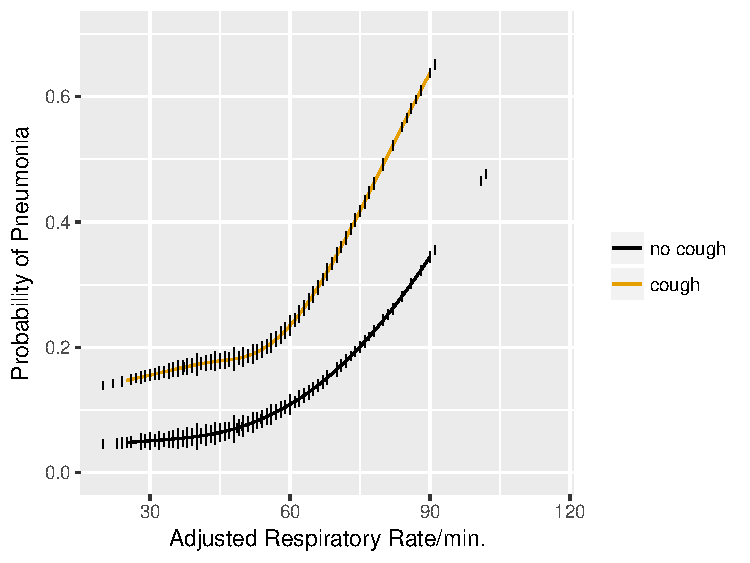
\includegraphics[width=\maxwidth]{info-pneuwho-1} }

\caption[Risk of pneumonia with two predictors]{Estimated risk of pneumonia with respect to two predictors in WHO ARI study from \citet{har98dev}.  Tick marks show data density of respiratory rate stratified by cough.  Any cutpoint for the rate \textbf{must} depend on cough to be consistent with optimum decision making, which must be risk-based.}\label{fig:info-pneuwho}
\end{figure}
\end{Schunk}
\clearpage
\subsection{What Kinds of True Thresholds Exist?}
\quoteit{Natura non facit saltus\\(Nature does not make jumps)}{Gottfried Wilhelm Leibniz}

\vspace{0.3in}

\textbf{Can Occur in Biology}\hfill \textbf{Cannot Occur \smaller Unless $X$=time}\\
{\smaller[2] Not Handled by Dichotomization}\hfill {\smaller[2] Assumed in Much of Biomarker Research}
\begin{Schunk}
\begin{figure}[htbp]

\centerline{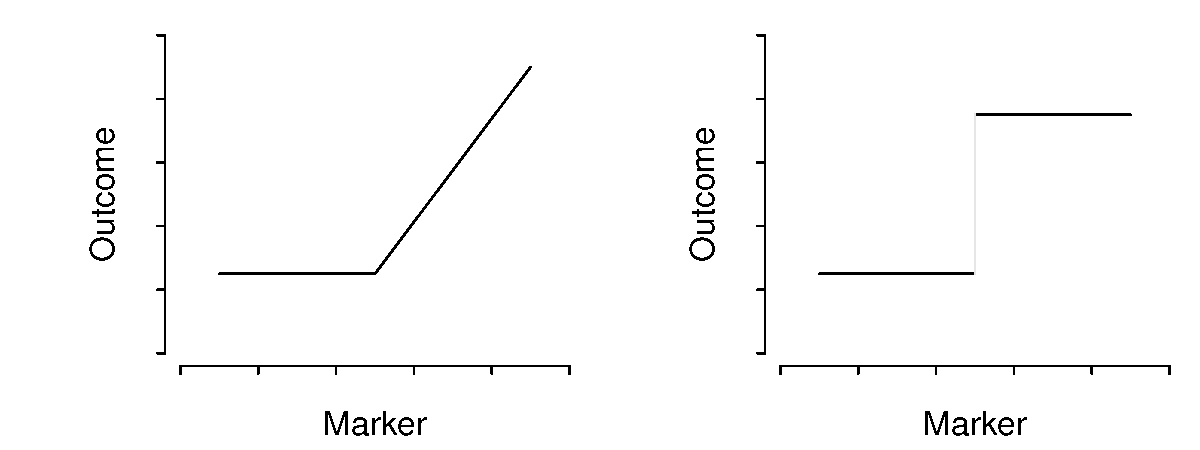
\includegraphics[width=\maxwidth]{info-thresholds-1} }

\caption[Two kinds of thresholds]{Two kinds of thresholds.  The pattern on the left represents a discontinuity in the first derivative (slope) of the function relating a marker to outcome.  On the right there is a lowest-order discontinuity.}\label{fig:info-thresholds}
\end{figure}
\end{Schunk}

\textbf{What Do Cutpoints Really Assume?}\\
Cutpoints assume discontinuous relationships of the type in the right
plot of Figure~\ref{fig:info-thresholds}, and they assume that the
true cutpoint is known.  Beyond the molecular level, such patterns do
not exist unless $X=$time and the discontinuity is caused by an event.
Cutpoints assume homogeneity of outcome on either side of the cutpoint.

\subsection{Cutpoints are Disasters}
\bi
\item Prognostic relevance of S-phase fraction in breast cancer:
19 different cutpoints used in literature
\item Cathepsin-D content and disease-free survival in node-negative
  breast cancer: 12 studies, 12 cutpoints
\item ASCO guidelines: neither cathepsin-D nor S-phrase fraction
recommended as prognostic markers~\citet{hol04con}
\ei

Cutpoints may be found that result in both increasing and
decreasing relationships with \textbf{any} dataset with zero
correlation

\centerline{\begin{tabular}{cc|cc} \\ \hline Range of Delay & Mean Score & Range of
  Delay & Mean Score \\ \hline
~0-11 & 210 & 0-3.8~~& 220 \\
11-20 & 215 & 3.8-8~~& 219 \\
21-30 & 217 & 8-113~~& 217 \\
31-40 & 218 & 113-170& 215 \\
41-~~ & 220 & 170-~~~& 210 \\ \hline
\end{tabular}}
\citet{wai06fin};~~See ``Dichotomania'' \citet{sen05dic} and
  \citet{roy06dic}

\centerline{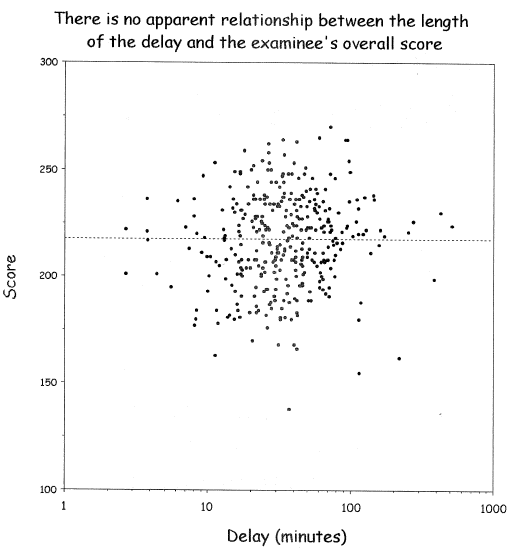
\includegraphics[height=4in]{wai06fin}}
\citet{wai06fin}

\textbf{In fact, virtually all published cutpoints are analysis
  artifacts} caused by finding a threshold that minimizes $P$-values
when comparing outcomes of subjects below with those above the
``threshold''.  Two-sample statistical tests suffer the least loss of
power when cutting at the median because this balances the sample
sizes.  That this method has nothing to do with biology can be readily
seen by adding observations on either tail of the marker, resulting in
a shift of the median toward that tail even though the relationship
between the continuous marker and the outcome remains unchanged.
\begin{center}\alabel{pg:info-gia14opt}
\includegraphics[width=0.7\textwidth]{fig2c.png}
\end{center}

 In ``positive'' studies: threshold 132--800 ng/L, correlation with study
    median $r=0.86$ (\citet{gia14opt})

\subsubsection{Lack of Meaning of Effects Based on Cutpoints}
\bi
\item Researchers often use cutpoints to estimate the high:low effects
  of risk factors (e.g., BMI vs.\ asthma)
\item Results in inaccurate predictions, residual confounding,
  impossible to interpret
\item high:low represents unknown mixtures of highs and lows
\item Effects (e.g., odds ratios) will vary with population
\item If the true effect is monotonic, adding subjects in the low
  range or high range or both will increase odds ratios (and all other
  effect measures) arbitrarily
\ei

\centerline{\includegraphics[width=0.7\textwidth]{roy06dicb.png}}
\citet{roy06dic},\citet{nag11ana},\citet{gia14opt}

Does a physician ask the nurse ``Is this patient's bilirubin $>$ 45''
or does she ask ``What is this patient's bilirubin level?''.
Imagine how a decision support system would trigger vastly different
decisions just because bilirubin was 46 instead of 44.

As an example of how a hazard ratio for a dichotomized continuous
predictor is an arbitrary function of the entire distribution of the
predictor within the two categories, consider a Cox model analysis of
simulated age where the true effect of age is linear.  First compute
the $\geq 50:< 50$ hazard ratio in all subjects, then in just the
subjects having age $< 60$, then in those with age $< 55$.  Then
repeat including all older subjects but excluding subjects with age
$\leq 40$.  Finally, compute the hazard ratio when only those age 40
to 60 are included.  Simulated times to events have an
exponential distribution, and proportional hazards holds.
\begin{Schunk}
\begin{Sinput}
set.seed(1)
n <- 1000
age <- rnorm(n, mean=50, sd=12)
describe(age)
\end{Sinput}
\begin{Soutput}
age 
       n  missing distinct     Info     Mean      Gmd      .05      .10 
    1000        0     1000        1    49.86    14.01    29.28    33.93 
     .25      .50      .75      .90      .95 
   41.63    49.58    58.26    65.89    70.93 

lowest : 13.90342 14.03661 14.72272 15.33295 18.84666
highest: 79.97194 81.79000 82.10889 86.66891 95.72332
\end{Soutput}
\begin{Sinput}
cens <- 15 * runif(n)
h  <- 0.02 * exp(0.04 * (age - 50))
dt <- -log(runif(n))/h
e  <- ifelse(dt <= cens,1,0)
dt <- pmin(dt, cens)
S  <- Surv(dt, e)
coef(cph(S ~ age))   # close to true value of 0.04 used in simulation
\end{Sinput}
\begin{Soutput}
       age 
0.04027519 
\end{Soutput}
\begin{Sinput}
exp(coef(cph(S ~ age >= 50)))   # >=50 : < 50 hazard ratio estimate
\end{Sinput}
\begin{Soutput}
     age 
2.148554 
\end{Soutput}
\begin{Sinput}
exp(coef(cph(S ~ age >= 50, subset=age < 60)))
\end{Sinput}
\begin{Soutput}
     age 
1.645141 
\end{Soutput}
\begin{Sinput}
exp(coef(cph(S ~ age >= 50, subset=age < 55)))
\end{Sinput}
\begin{Soutput}
     age 
1.461928 
\end{Soutput}
\begin{Sinput}
exp(coef(cph(S ~ age >= 50, subset=age > 40)))
\end{Sinput}
\begin{Soutput}
     age 
1.760201 
\end{Soutput}
\begin{Sinput}
exp(coef(cph(S ~ age >= 50, subset=age > 40 & age < 60)))
\end{Sinput}
\begin{Soutput}
     age 
1.354001 
\end{Soutput}
\end{Schunk}

See
\href{https://bmcmedresmethodol.biomedcentral.com/articles/10.1186/1471-2288-12-21}{this} 
for excellent graphical examples of the harm of categorizing
predictors, especially when using quantile groups.

\subsection{Categorizing Outcomes}\alabel{sec:info-catoutcomes}
\bi
\item Arbitrary, low power, can be difficult to interpret
\item Example: ``The treatment is called successful if either the
  patient has gone down from a baseline diastolic blood pressure of
  $\geq 95$ mmHg to $\leq 90$ mmHg or has achieved a 10\% reduction in
  blood pressure from baseline.''
\item Senn derived the response probabililty function for this
  discontinuous concocted endpoint
\ei

\centerline{\includegraphics[height=.35\textheight]{dichotomaniaFig3.png}}
\citet{sen05dic} after Goetghebeur [1998]

Is a mean difference of 5.4mmHg more difficult to interpret than
A:17\% vs.\ B:22\% hit clinical target?

``Responder'' analysis in clinical trials results in huge information loss and arbitrariness.  Some issue:
\bi
\item Responder analyses use cutpoints on continuous or ordinal variables and cite earlier data supporting their choice of cutpoints.  No example has been produced where the earlier data actually support the cutpoint.
\item Many responder analyses are based on change scores when they should be based solely on the follow-up outcome variable, adjusted for baseline as a covariate.
\item The cutpoints are always arbitrary.
\item There is a huge power loss (see Section~\ref{sec:info-catoutcomes}).
\item The responder probability is often a function of variables that one does not want it to be a function of (see graph above).
\ei


\citet{fed09con} is one of the best papers quantifying the information
and power loss from categorizing continuous outcomes.  One of their
examples is that a clinical trial of 100 subjects with continuous $Y$
is statistically equivalent to a trial of 158 dichotomized
observations, assuming that the dichotomization is at the
\textbf{optimum} point (the population median).  They show that it is
very easy for dichotomization of $Y$ to raise the needed sample size
by a factor of 5.

\centerline{\includegraphics[width=\textwidth]{fed09conFig1}}\alabel{pg:info-fed09con}
\citet{fed09con}


\subsection{Classification vs.\ Probabilistic Thinking}%
\movie{https://youtu.be/1yYrDVN_AYc}
\quoteit{\textbf{Number needed to treat}. The only way, we are told,
  that physicians can understand probabilities: odds being a difficult
  concept only comprehensible to statisticians, bookies, punters and
  readers of the sports pages of popular newspapers.}{\citet{sensta}}

\bi
\item Many studies attempt to classify patients as diseased/normal
\item Given a reliable estimate of the probability of disease and the
  consequences of +/- one can make an optimal decision
\item Consequences are known at the point of care, not by the authors;
categorization \textbf{only} at point of care
\item Continuous probabilities are self-contained, with their own
  ``error rates''
\item Middle probs.\ allow for ``gray zone'', deferred decision
\ei
\centerline{\begin{tabular}{cccc}\hline
Patient & Prob[disease] & Decision & Prob[error] \\ \hline
1       &   0.03        & normal   & 0.03 \\
2       &   0.40        & normal   & 0.40 \\
3       &   0.75        & disease  & 0.25 \\ \hline
\end{tabular}
}

Note that much of diagnostic research seems to be aimed at
making optimum decisions for groups of patients.  The optimum decision
for a group (if such a concept even has meaning) is not optimum for
individuals in the group.



\subsection{Components of Optimal Decisions}
\centerline{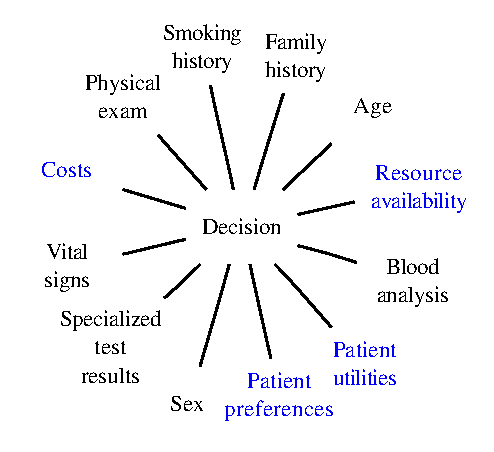
\includegraphics[height=0.4\textheight]{mdDec}}

Statistical models reduce the dimensionality of the problem \emph{but
    not to unity}

\centerline{\includegraphics[height=0.4\textheight]{mdDecm}}

\section{Problems with Classification of Predictions}%
\movie{https://youtu.be/FDTwEZ3KcyA}
\bi
\item Feature selection / predictive model building requires choice of
a scoring rule, e.g.\ correlation coefficient or proportion of correct
classifications
\item Prop.\ classified correctly is a discontinuous \textbf{improper scoring
    rule}
 \bi
 \item Maximized by bogus model \smaller{(example below)}
 \ei
\item Minimum information
 \bi
 \item low statistical power
 \item high standard errors of regression coefficients
 \item arbitrary to choice of cutoff on predicted risk
 \item forces binary decision, does not yield a ``gray zone''
   $\rightarrow$ more data needed
 \ei
\item Takes analyst to be provider of utility function and not the
 treating physician
\item Sensitivity and specificity are also improper scoring rules
\ei


\subsection{Example: Damage Caused by Improper Scoring Rule}
\bi
\item Predicting probability of an event, e.g., Prob[disease]
\item $N=400$, 0.57 of subjects have disease
\item Classify as diseased if prob.\ $>0.5$
\ei
\begin{center}\begin{tabular}{lccc}\hline
Model & $c$   & $\chi^{2}$ & Proportion \\
      & Index &            & Correct \\ \hline
age     & .592 & 10.5 & .622\\
sex     & .589 & 12.4 & .588\\
age+sex & .639 & 22.8 & .600\\
constant &.500 & ~0.0 & .573\\ \hline
\end{tabular}\end{center}

Adjusted Odds Ratios:\\
\begin{tabular}{ll}
age (IQR 58y:42y) & 1.6 (0.95CL 1.2-2.0)\\
sex (f:m)         & 0.5 (0.95CL 0.3-0.7)\\
\end{tabular}

Test of sex effect adjusted for age $(22.8-10.5)$:\\$P=0.0005$

\subsubsection{Example where an improper accuracy score resulted in incorrect original analyses and incorrect re-analysis}
\citet{mic05pre} used an improper accuracy score (proportion
classified ``correctly'') and
claimed there was really no signal in all the published gene
microarray studies they could analyze.  This is true from the
standpoint of repeating the original analyses (which also used improper
accuracy scores) using multiple splits of the data, exposing the
fallacy of using single data-splitting for validation.  \citet{ali09fac}
used a semi-proper accuracy score ($c$-index) and they repeated 10-fold
cross-validation 100 times instead of using highly volatile data
splitting.  They showed that the gene microarrays did indeed have
predictive signals.\footnote{\citet{ali09fac} also used correct
  statistical models for time-to-event data that properly accounted
  for variable follow-up/censoring.}

\centerline{\begin{tabular}{l|l}
\citet{mic05pre} & \citet{ali09fac} \\ \hline
\% classified correctly & $c$-index\\
Single split-sample validation & Multiple repeats of 10-fold CV\\
Wrong tests & Correct tests\\
~~(censoring, failure times) & \\ \hline
5 of 7 published microarray & 6 of 7 have signals\\
~~studies had no signal & \\
\end{tabular}}

\section{Value of Continuous Markers}
\bi
\item Avoid arbitrary cutpoints
\item Better risk spectrum
\item Provides gray zone
\item Increases power/precision
\ei

\subsection{Prognosis in Prostate Cancer}
\begin{Schunk}
\begin{Sinput}
load('~/doc/Talks/infoAllergy/kattan.rda')
attach(kattan)
t   <- t.stg
gs  <- bx.glsn
psa <- preop.psa
t12 <- t.stg %in% Cs(T1C,T2A,T2B,T2C)

s <- score.binary(t12 & gs<=6 & psa<10,
                  t12 & gs<=6 & psa >=10 & psa < 20,
                  t12 & gs==7 & psa < 20,
                  (t12 & gs<=6 & psa>=20) |
                  (t12 & gs>=8 & psa<20),
                  t12 & gs>=7 & psa>=20,
                  t.stg=='T3')
levels(s) <- c('none','I', 'IIA', 'IIB', 'IIIA', 'IIIB', 'IIIC')
u <- is.na(psa + gs) | is.na(t.stg)
s[s=='none'] <- NA
s <- s[drop=TRUE]
s3 <- s
levels(s3) <- c('I','II','II','III','III','III')
table(s3)
\end{Sinput}
\begin{Soutput}
s3
   I   II  III 
1108  607  271 
\end{Soutput}
\begin{Sinput}
units(time.event) <- 'month'
dd <- datadist(data.frame(psa, gs)); options(datadist='dd')
S <- Surv(time.event, event=='YES')
label(psa) <- 'PSA'; label(gs) <- 'Gleason Score'
f <- cph(S ~ rcs(sqrt(psa), 4), surv=TRUE, x=TRUE, y=TRUE)
p <- Predict(f, psa, time=24, fun=function(x) 1 - x)
h <- cph(S ~ s3, surv=TRUE)
z <- 1 - survest(h, times=24)$surv
\end{Sinput}
\begin{Sinput}
ggplot(p, rdata=data.frame(psa), ylab='2-year Disease Recurrence Risk') +
  geom_hline(yintercept=unique(z), col='red', size=0.2)   # Fig. (*\ref{fig:info-psa}*)
\end{Sinput}
\begin{figure}[htbp]

\centerline{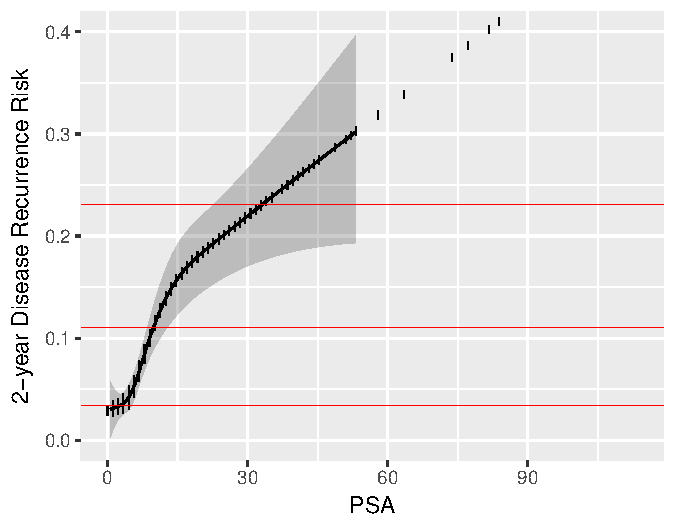
\includegraphics[width=\maxwidth]{info-psa-1} }

\caption[Continuous PSA vs. risk]{Relationship between post-op PSA level and 2-year recurrence risk.  Horizontal lines represent the only prognoses provided by the new staging system. Data are courtesy of M Kattan from JNCI 98:715; 2006.  Modification of AJCC staging by Roach \emph{et al.} 2006.}\label{fig:info-psa}
\end{figure}
\end{Schunk}

Now examine the entire spectrum of estimated prognoses from variables
models and from discontinuous staging systems.

\begin{Schunk}
\begin{Sinput}
f <- cph(S ~ rcs(sqrt(psa),4) + pol(gs,2), surv=TRUE)
g <- function(form, lab) {
  f <- cph(form, surv=TRUE, subset=!u)
  cat(lab,'\n'); print(coef(f))
  s <- f$stats
  cat('N:', s['Obs'],'\tL.R.:', round(s['Model L.R.'],1),
      '\td.f.:',s['d.f.'],'\n\n')
  prob24 <- 1 - survest(f, times=24)$surv
  prn(sum(!is.na(prob24)))
  p2 <<- c(p2, prob24[2])  # save est. prognosis for one subject
  p1936 <<- c(p1936, prob24[1936])
  C <- rcorr.cens(1-prob24, S[!u,])['C Index']
  data.frame(model=lab, chisq=s['Model L.R.'], d.f.=s['d.f.'],
             C=C, prognosis=prob24)
}
p2 <- p1936 <- NULL
w <-          g(S ~ t.stg, 'Old Stage')
\end{Sinput}
\begin{Soutput}
Old Stage 
t.stg=T2A t.stg=T2B t.stg=T2C  t.stg=T3 
0.2791987 1.2377218 1.0626197 1.7681393 
N: 1978 	L.R.: 70.5 	d.f.: 4 
\end{Soutput}
\begin{Soutput}

sum(!is.na(prob24))

[1] 1978
\end{Soutput}
\begin{Sinput}
w <- rbind(w, g(S ~ s3, 'New Stage'))
\end{Sinput}
\begin{Soutput}
New Stage 
   s3=II   s3=III 
1.225296 1.990355 
N: 1978 	L.R.: 135.8 	d.f.: 2 
\end{Soutput}
\begin{Soutput}

sum(!is.na(prob24))

[1] 1978
\end{Soutput}
\begin{Sinput}
w <- rbind(w, g(S ~ s, 'New Stage, 6 Levels'))
\end{Sinput}
\begin{Soutput}
New Stage, 6 Levels 
   s=IIA    s=IIB   s=IIIA   s=IIIB   s=IIIC 
1.181824 1.248864 1.829265 2.410810 1.954420 
N: 1978 	L.R.: 140.3 	d.f.: 5 
\end{Soutput}
\begin{Soutput}

sum(!is.na(prob24))

[1] 1978
\end{Soutput}
\begin{Sinput}
w <- rbind(w, g(S ~ pol(gs,2),        'Gleason'))
\end{Sinput}
\begin{Soutput}
Gleason 
         gs        gs^2 
-0.42563792  0.07857747 
N: 1978 	L.R.: 90.3 	d.f.: 2 
\end{Soutput}
\begin{Soutput}

sum(!is.na(prob24))

[1] 1978
\end{Soutput}
\begin{Sinput}
w <- rbind(w, g(S ~ rcs(sqrt(psa),4), 'PSA'))
\end{Sinput}
\begin{Soutput}
PSA 
         psa         psa'        psa'' 
 -0.09621478   4.07465107 -14.86458188 
N: 1978 	L.R.: 95.3 	d.f.: 3 
\end{Soutput}
\begin{Soutput}

sum(!is.na(prob24))

[1] 1978
\end{Soutput}
\begin{Sinput}
w <- rbind(w, g(S ~ rcs(sqrt(psa),4) + pol(gs,2), 'PSA+Gleason'))
\end{Sinput}
\begin{Soutput}
PSA+Gleason 
         psa         psa'        psa''           gs         gs^2 
 -0.11703664   3.37768454 -12.04890937  -0.20429572   0.05458832 
N: 1978 	L.R.: 160.2 	d.f.: 5 
\end{Soutput}
\begin{Soutput}

sum(!is.na(prob24))

[1] 1978
\end{Soutput}
\begin{Sinput}
w <- rbind(w, g(S ~ rcs(sqrt(psa),4) + pol(gs,2) + t.stg,
                'PSA+Gleason+Old Stage'))
\end{Sinput}
\begin{Soutput}
PSA+Gleason+Old Stage 
        psa        psa'       psa''          gs        gs^2   t.stg=T2A 
 0.12361025  2.26959366 -8.62949512 -0.01467426  0.03511191  0.27334309 
  t.stg=T2B   t.stg=T2C    t.stg=T3 
 0.93943683  0.69083735  1.07508642 
N: 1978 	L.R.: 187 	d.f.: 9 
\end{Soutput}
\begin{Soutput}

sum(!is.na(prob24))

[1] 1978
\end{Soutput}
\begin{Sinput}
w$z <- paste(w$model, '\n',
             'X2-d.f.=',round(w$chisq-w$d.f.),
             '  C=', sprintf("%.2f", w$C), sep='')
w$z <- with(w, factor(z, unique(z)))
require(lattice)
stripplot(z ~ prognosis, data=w, lwd=1.5,    # Fig. (*\ref{fig:info-spectrum}*)
          panel=function(x, y, ...) {
            llines(p2, 1:7, col=gray(.6))
            ## llines(p1936, 1:7, col=gray(.8), lwd=2)
            ## panel.stripplot(x, y, ..., jitter.data=TRUE, cex=.5)
            for(iy in unique(unclass(y))) {
              s <- unclass(y)==iy
              histSpike(x[s], y=rep(iy,sum(s)), add=TRUE, grid=TRUE)
            }
            panel.abline(v=0, col=gray(.7))
          },
          xlab='Predicted 2-year\nDisease Recurrence Probability')
\end{Sinput}
\begin{figure}[htbp]

\centerline{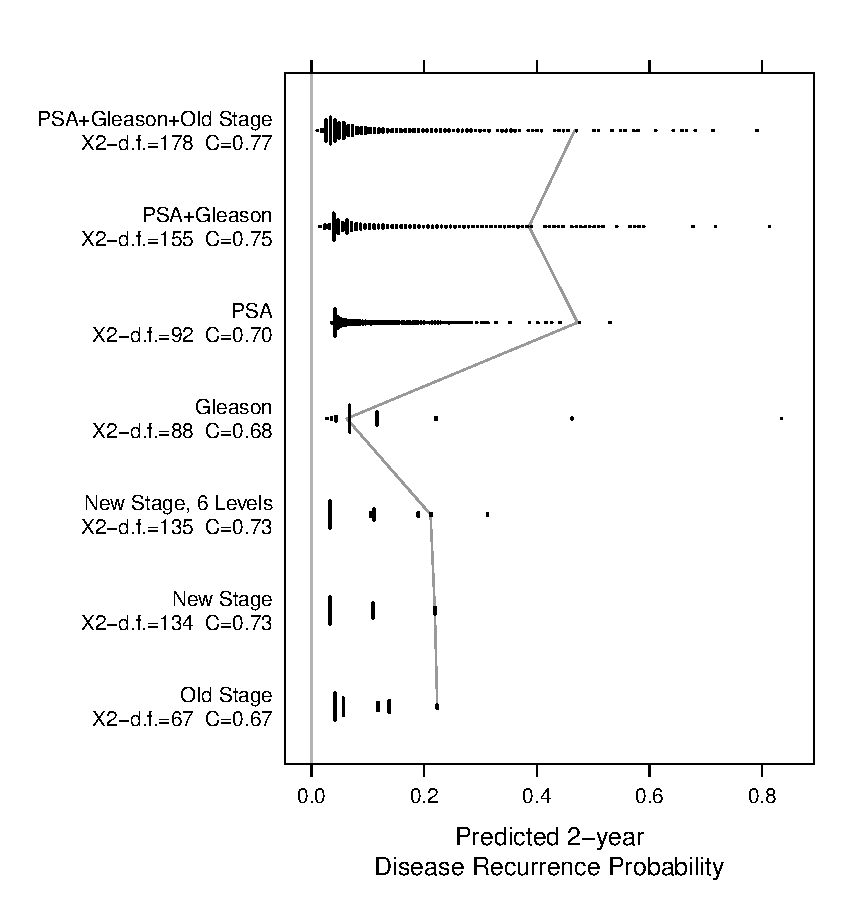
\includegraphics[width=\maxwidth]{info-spectrum-1} }

\caption[Prognostic spectrum from various models]{Prognostic spectrum from various models with model $\chi^2$ - d.f., and generalized $c$-index.  The mostly vertical segmented line connects different prognostic estimates for the same man.}\label{fig:info-spectrum}
\end{figure}
\end{Schunk}
\clearpage
\section{Harm from Ignoring Information}
\subsection{Case Study: Cardiac Anti-arrhythmic Drugs}\label{sec:pvcs}
\bi
\item Premature ventricular contractions were observed in patients
surviving acute myocardial infarction
\item Frequent PVCs $\uparrow$ incidence of sudden death
\ei

\centerline{\includegraphics[height=0.2\textheight,width=\textwidth]{pvcDeadlyMedicine.png}}
\citet{moo95dea}, p.\ 46

\textbf{Arrhythmia Suppression Hypothesis}

\quoteit{Any prophylactic program against sudden death must involve
  the use of anti-arrhythmic drugs to subdue ventricular premature
  complexes.}{Bernard Lown\\ {\smaller Widely accepted by 1978}}

\centerline{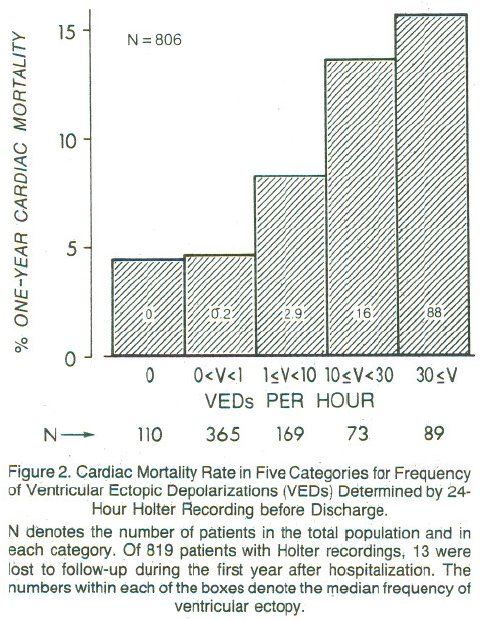
\includegraphics[height=.5\textheight]{mul83risFig2.jpg}}
\citet{moo95dea}, p.~49; \cite{mul83ris}

Are PVCs independent risk factors for sudden cardiac death?

Researchers developed a 4-variable model for prognosis after acute MI
 \bi
 \item left ventricular ejection fraction (EF) $< 0.4$
 \item PVCs $>$ 10/hr
 \item Lung rales
 \item Heart failure class II,III,IV
 \ei

\centerline{\includegraphics[height=.5\textheight]{mul83risFig3b.jpg}}
\citet{mul83ris}

\textbf{Dichotomania Caused Severe Problems}
\bi
\item EF alone provides same prognostic spectrum as the researchers'
model
\item Did not adjust for EF!; PVCs $\uparrow$ when EF$<0.2$
\item Arrhythmias prognostic in isolation, not after
adjustment for continuous EF and anatomic variables
\item Arrhythmias predicted by local contraction
abnorm., then global function (EF)
\ei

\centerline{\includegraphics[width=0.6\textwidth]{mul83risFig1.jpg}}
\citet{mul83ris}; \citet{cal82pro}

\subsection{CAST: Cardiac Arrhythmia Suppression Trial}
\bi
\item Randomized placebo, moricizine, and Class IC anti-arrhythmic
drugs flecainide and encainide
\item Cardiologists: unethical to randomize to placebo
\item Placebo group included after vigorous argument
\item Tests design as one-tailed; did not entertain possibility of
harm
\item Data and Safety Monitoring Board recommended early termination
of flecainide and encainide arms
\item Deaths $\frac{56}{730}$ drug, $\frac{22}{725}$ placebo, RR 2.5
\ei
\citet{car89pre}

\textbf{Conclusions: Class I Anti-Arrhythmics}

\centerline{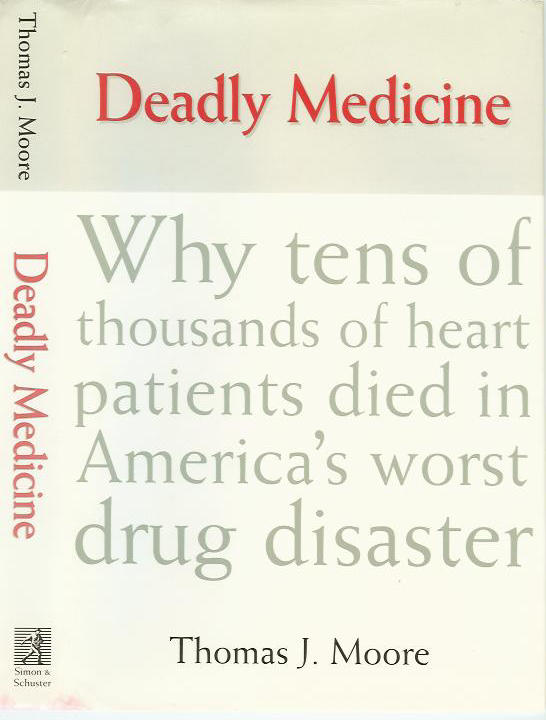
\includegraphics[height=.3\textheight]{deadlyMedicine.jpg}}

Estimate of excess deaths from Class I anti-arrhythmic drugs: 24,000--69,000\\
Estimate of excess deaths from Vioxx: 27,000--55,000

Arrhythmia suppression hypothesis refuted; PVCs merely indicators of
underlying, permanent damage

\citet{moo95dea}, pp.~289,49; D Graham, FDA

\section{Case Study in Faulty Dichotomization of a Clinical Outcome: Statistical and Ethical Concerns in Clinical Trials for
  Crohn's Disease}\alabel{sec:crohn}

\subsection{Background}
Many clinical trials are underway for studying treatments for Crohn's disease.
The primary endpoint for these studies is a
discontinuous, information--losing transformation of the Crohn's
Disease Activity Index
(CDAI)~\cite{bes76dev}, which  was developed in 1976 by
using an exploratory stepwise regression method to predict four levels
of clinicians' impressions of patients' current
status\footnote{Ordinary least squares regression was used for the
  ordinal response variable.  The levels of the response were assumed
  to be equally spaced in severity on a numerical
  scale of 1, 3, 5, 7 with no justification.}.  The first
level (``very well'') was assumed to indicate the patient was in
remission.  The model was overfitted and was not validated.  The
model's coefficients were scaled and rounded, resulting in the
following scoring system (see \url{http://www.ibdjohn.com/cdai}).
\clearpage
\begin{center}
\includegraphics[width=.7\textwidth]{score1.png}\\
\includegraphics[width=.7\textwidth]{score2.png}
\end{center}

The original authors plotted the predicted scores against the four
clinical categories as shown below.

\centerline{\includegraphics[width=.7\textwidth]{bes76devFig1.png}}

The authors arbitrarily assigned a cutoff of 150, below which
indicates ``remission.''\footnote{However, the authors intended for
  CDAI to be used on a continuum: ``\ldots a numerical index was
  needed, the numerical value of which would be proportional to degree
  of illness \ldots it could be used as the principal measure of
  response to the therapy under trial \ldots the CDAI appears to meet
  those needs. \ldots The data presented \ldots is an accurate
  numerical expression of the physician's over-all assessment of
  degree of illness in a large group of patients \ldots we believe
  that it should be useful to all physicians who treat Crohn's disease
  as a method of assessing patient progress.''.}  It can be seen that
``remission'' includes a
good number of patients actually classified as ``fair to good'' or
``poor.''  A cutoff only exists when there is a break in the
distribution of scores.  As an example, data were simulated from a
population in which every patient having a score below 100 had a
probability of response of 0.2 and every patient having a score above
100 had a probability of response of 0.8.  Histograms showing the
distributions of non-responders (just above the $x$-axis) and
responders (at the top of the graph) appear in the figure below.  A
flexibly fitted logistic regression model relating observed scores to
actual response status is shown, along with 0.95 confidence intervals
for the fit.

\begin{Schunk}
\begin{Sinput}
require(rms)
set.seed(4)
n <- 900
X <- rnorm(n, 100, 20)
dd <- datadist(X); options(datadist='dd')

p <- ifelse(X < 100, .2, .8)
y <- ifelse(runif(n) <= p, 1, 0)

f <- lrm(y ~ rcs(X, c(90,95,100,105,110)))
hs <- function(yval, side)
  histSpikeg(yhat ~ X, data=subset(data.frame(X, y), y == yval),
             side = side, ylim = c(0, 1),
             frac = function(f) .03 * f / max(f))
ggplot(Predict(f, fun=plogis), ylab='Probability of Response') +
  hs(0, 1) + hs(1, 3) + geom_vline(xintercept=100, col=gray(.7))
\end{Sinput}


\centerline{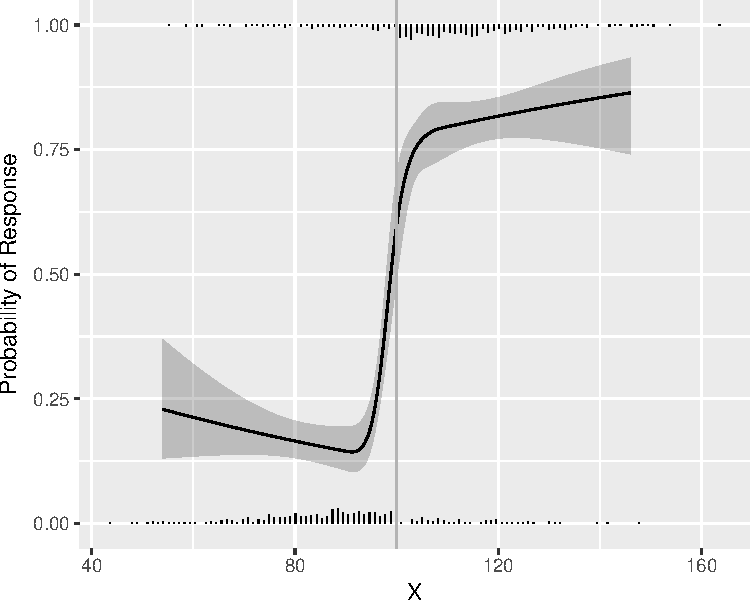
\includegraphics[width=\maxwidth]{info-cutpointExists-1} }

\end{Schunk}

One can see that the fitted curves justify the use of a cut-point of
100.  However, the original scores from the development of CDAI do not
justify the existence of a cutoff.  The fitted logistic model used to
relate ``very well'' to the other three categories is shown below.


\begin{Schunk}
\begin{Sinput}
# Points from published graph were defined in code not printed
g <- trunc(d$x)
g <- factor(g, 0:3, c('very well', 'fair to good', 'poor', 'very poor'))
remiss <- 1 * (g == 'very well')
CDAI <- d$y
label(CDAI) <- "Crohn's Disease Activity Index"
label(remiss) <- 'Remission'
dd <- datadist(CDAI,remiss); options(datadist='dd')
f <- lrm(remiss ~ rcs(CDAI,4))
ggplot(Predict(f, fun=plogis), ylab='Probability of Remission')
\end{Sinput}


\centerline{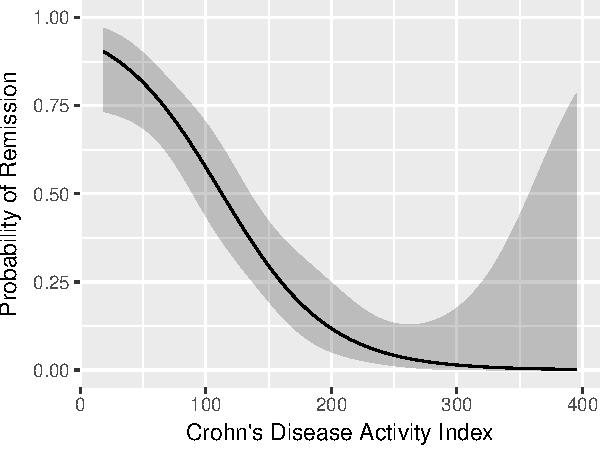
\includegraphics[width=\maxwidth]{info-devlogist-1} }

\end{Schunk}

It is readily seen that no cutoff exists, and one would have to be
below CDAI of 100 for the probability of remission to fall below even
0.5.  The probability does not exceed 0.9 until the score falls below
25.  Thus there is no clinical justification for the 150 cut-point.

\subsection{Loss of Information from Using Cut-points}
The statistical analysis plan in the Crohn's disease protocols specify
that efficacy will be judged by comparing two proportions after
classifying patients' CDAIs as above or below the cutoff of 150.
Even if one could justify a certain cutoff from the data, the use of the
cutoff is usually not warranted.  This is because of the huge loss of
statistical efficiency, precision, and power from dichotomizing
continuous variables as discussed in more detail in
Section~\ref{sec:info-catoutcomes}.
If one were forced to dichotomize a continuous
response $Y$, the cut-point that loses the least efficiency is the
population median of $Y$ combining treatment groups.  That implies a
statistical efficiency of $\frac{2}{\pi}$ or 0.637 when compared to
the efficient two-sample $t$-test if the data are normally
distributed\footnote{Note that the efficiency of the Wilcoxon test
  compared to the $t$-test is $\frac{3}{\pi}$ and the efficiency of
  the sign test compared to the $t$-test is $\frac{2}{\pi}$.  Had
  analysis of covariance been used instead of a simple two-group
  comparison, the baseline level of CDAI could have been adjusted for
  as a covariate.  This would have increased the power of the
  continuous scale approach to even higher levels.}.  In other words,
the optimum cut-point would require
studying 158 patients after dichotomizing the response variable to get
the same power as analyzing the continuous response variable in 100
patients.

\subsection{Ethical Concerns and Summary}
The CDAI was based on a sloppily-fit regression model predicting a
subjective clinical impression.  Then a cutoff of 150 was used to
classify patients as in remission or not.  The choice of this cutoff
is in opposition to the data used to support it.  The data show that
one must have CDAI below 100 to have a chance of remission of only
0.5.  Hence the use of CDAI$<150$ as a clinical endpoint was
based on a faulty premise that apparently has never been investigated
in the Crohn's disease research community.   CDAI can
easily be analyzed as a continuous variable, preserving all of
the power of the statistical test for efficacy (e.g., two-sample
$t$-test).  The results of the $t$-test can readily be translated to
estimate any clinical ``success probability'' of interest, using
efficient maximum likelihood estimators\footnote{Given $\bar{x}$ and
  $s$ as estimates of $\mu$ and $\sigma$, the estimate of the
  probability that CDAI $< 150$ is simply $\Phi(\frac{150-\bar{x}}{s})$, where
  $\Phi$ is the cumulative distribution function of the standard
  normal distribution.  For example, if the observed mean were 150, we
would estimate the probability of remission to be 0.5.}

There are substantial ethical questions that ought to be addressed
when statistical power is wasted:
\begin{enumerate}
\item Patients are not consenting to be put at risk for a trial that
  doesn't yield valid results.
\item A rigorous scientific approach is necessary in order to allow
  enrollment of individuals as subjects in research.
\item Investigators are obligated to reduce the number of subjects
  exposed to harm and the amount of harm to which each subject is
  exposed.
\end{enumerate}
It is not known whether investigators are receiving per-patient
payments for studies in which sample size is inflated by dichotomizing
CDAI.

\section{Information May Sometimes Be Costly}
\quoteit{When the Missionaries arrived, the Africans had the Land and
  the Missionaries had the Bible. They taught how to pray with our
  eyes closed. When we opened them, they had the land and we had the
  Bible.}{Jomo Kenyatta, founding father of Kenya; also attributed to
  Desmond Tutu}

\quoteit{Information itself has a liberal bias.}{The Colbert Report\\2006-11-28}
\nocite{bor07sta,bri08ski,vic08dec}
\vspace{-2in}
{\smaller[3]../../Talks/infoAllergy/abstract.tex}
